\subsection{Election November 3, 1936: *Roosevelt vs Landon}
\begin{frame}[t]{Election November 3, 1936: *Franklin Roosevelt}
\small

\begin{columns}[T, onlytextwidth]
\column{0.48\textwidth}
\vspace{-1em}
{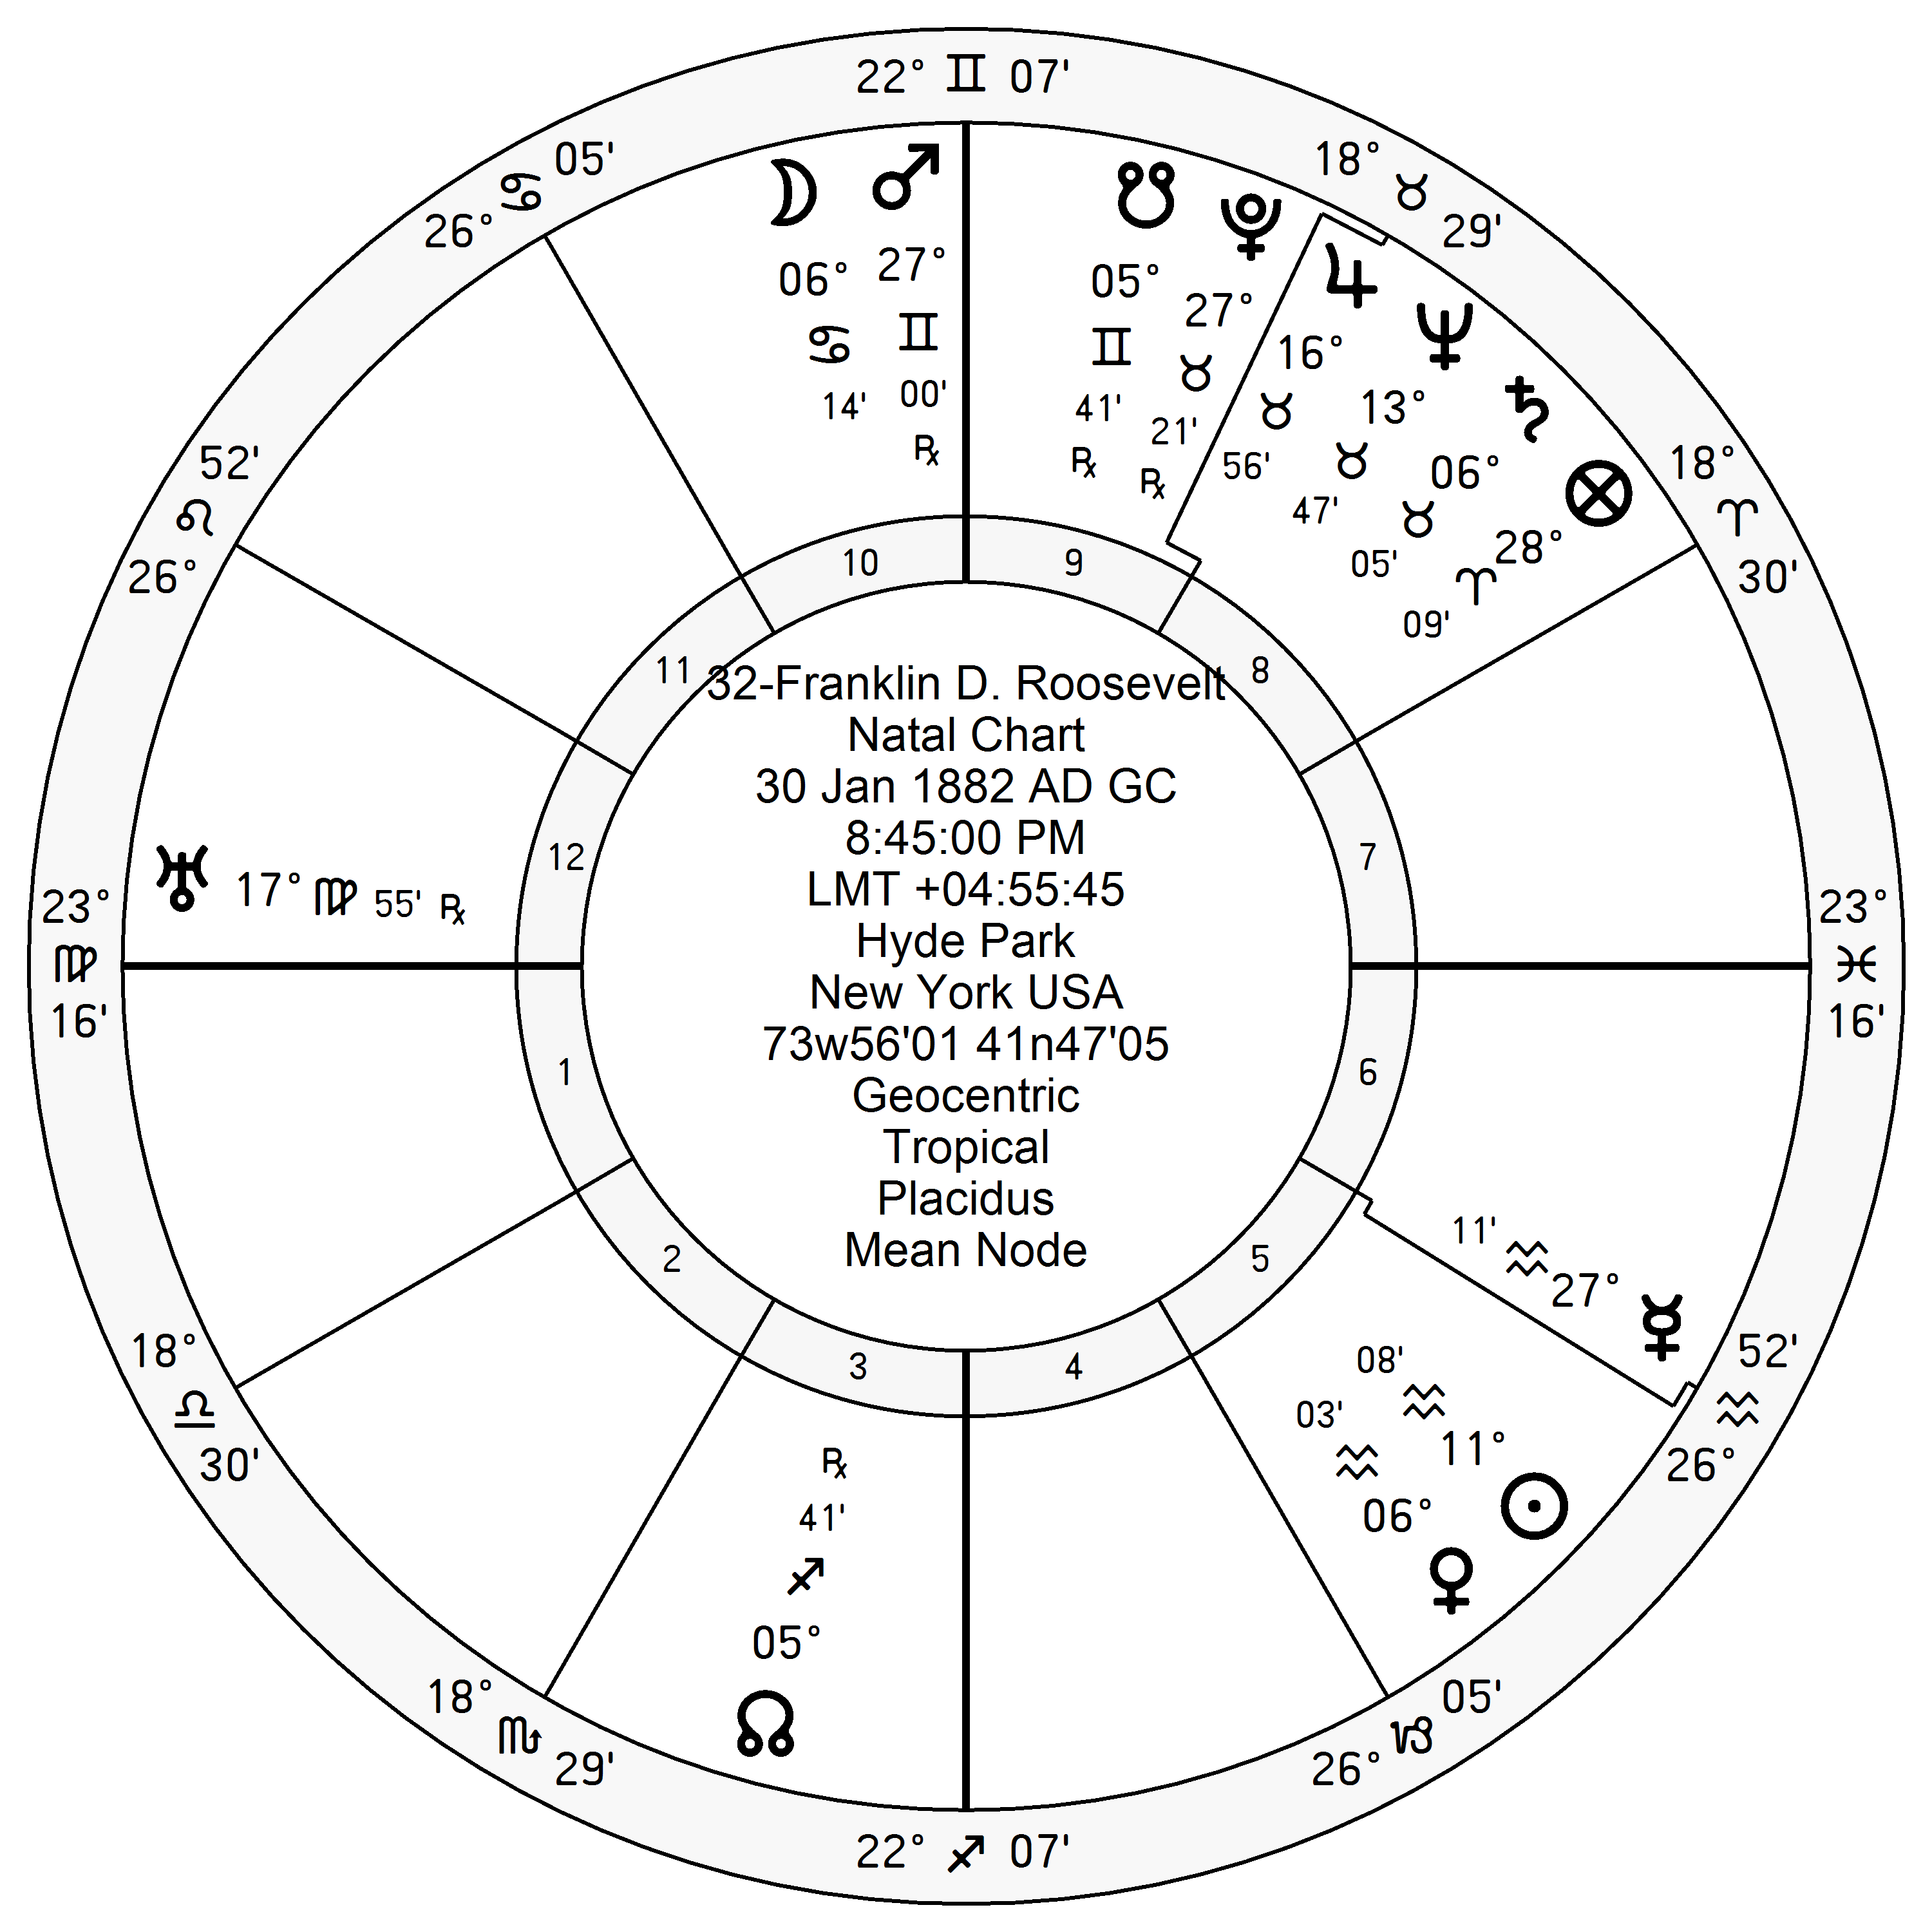
\includegraphics[width=0.9\textwidth]{charts/FDR.png}}
\fontsize{7pt}{8pt}\selectfont

\Jupiter\, \Trine\, P10, \Sextile\, N10, P1; in a mitigated \Quincunx\, (\Opposition) with N1 which appears to have been enough for the win as his opponent has only one hard aspect involving a burnt \Mercury.

\column{0.48\textwidth}
\vspace{-1em}
{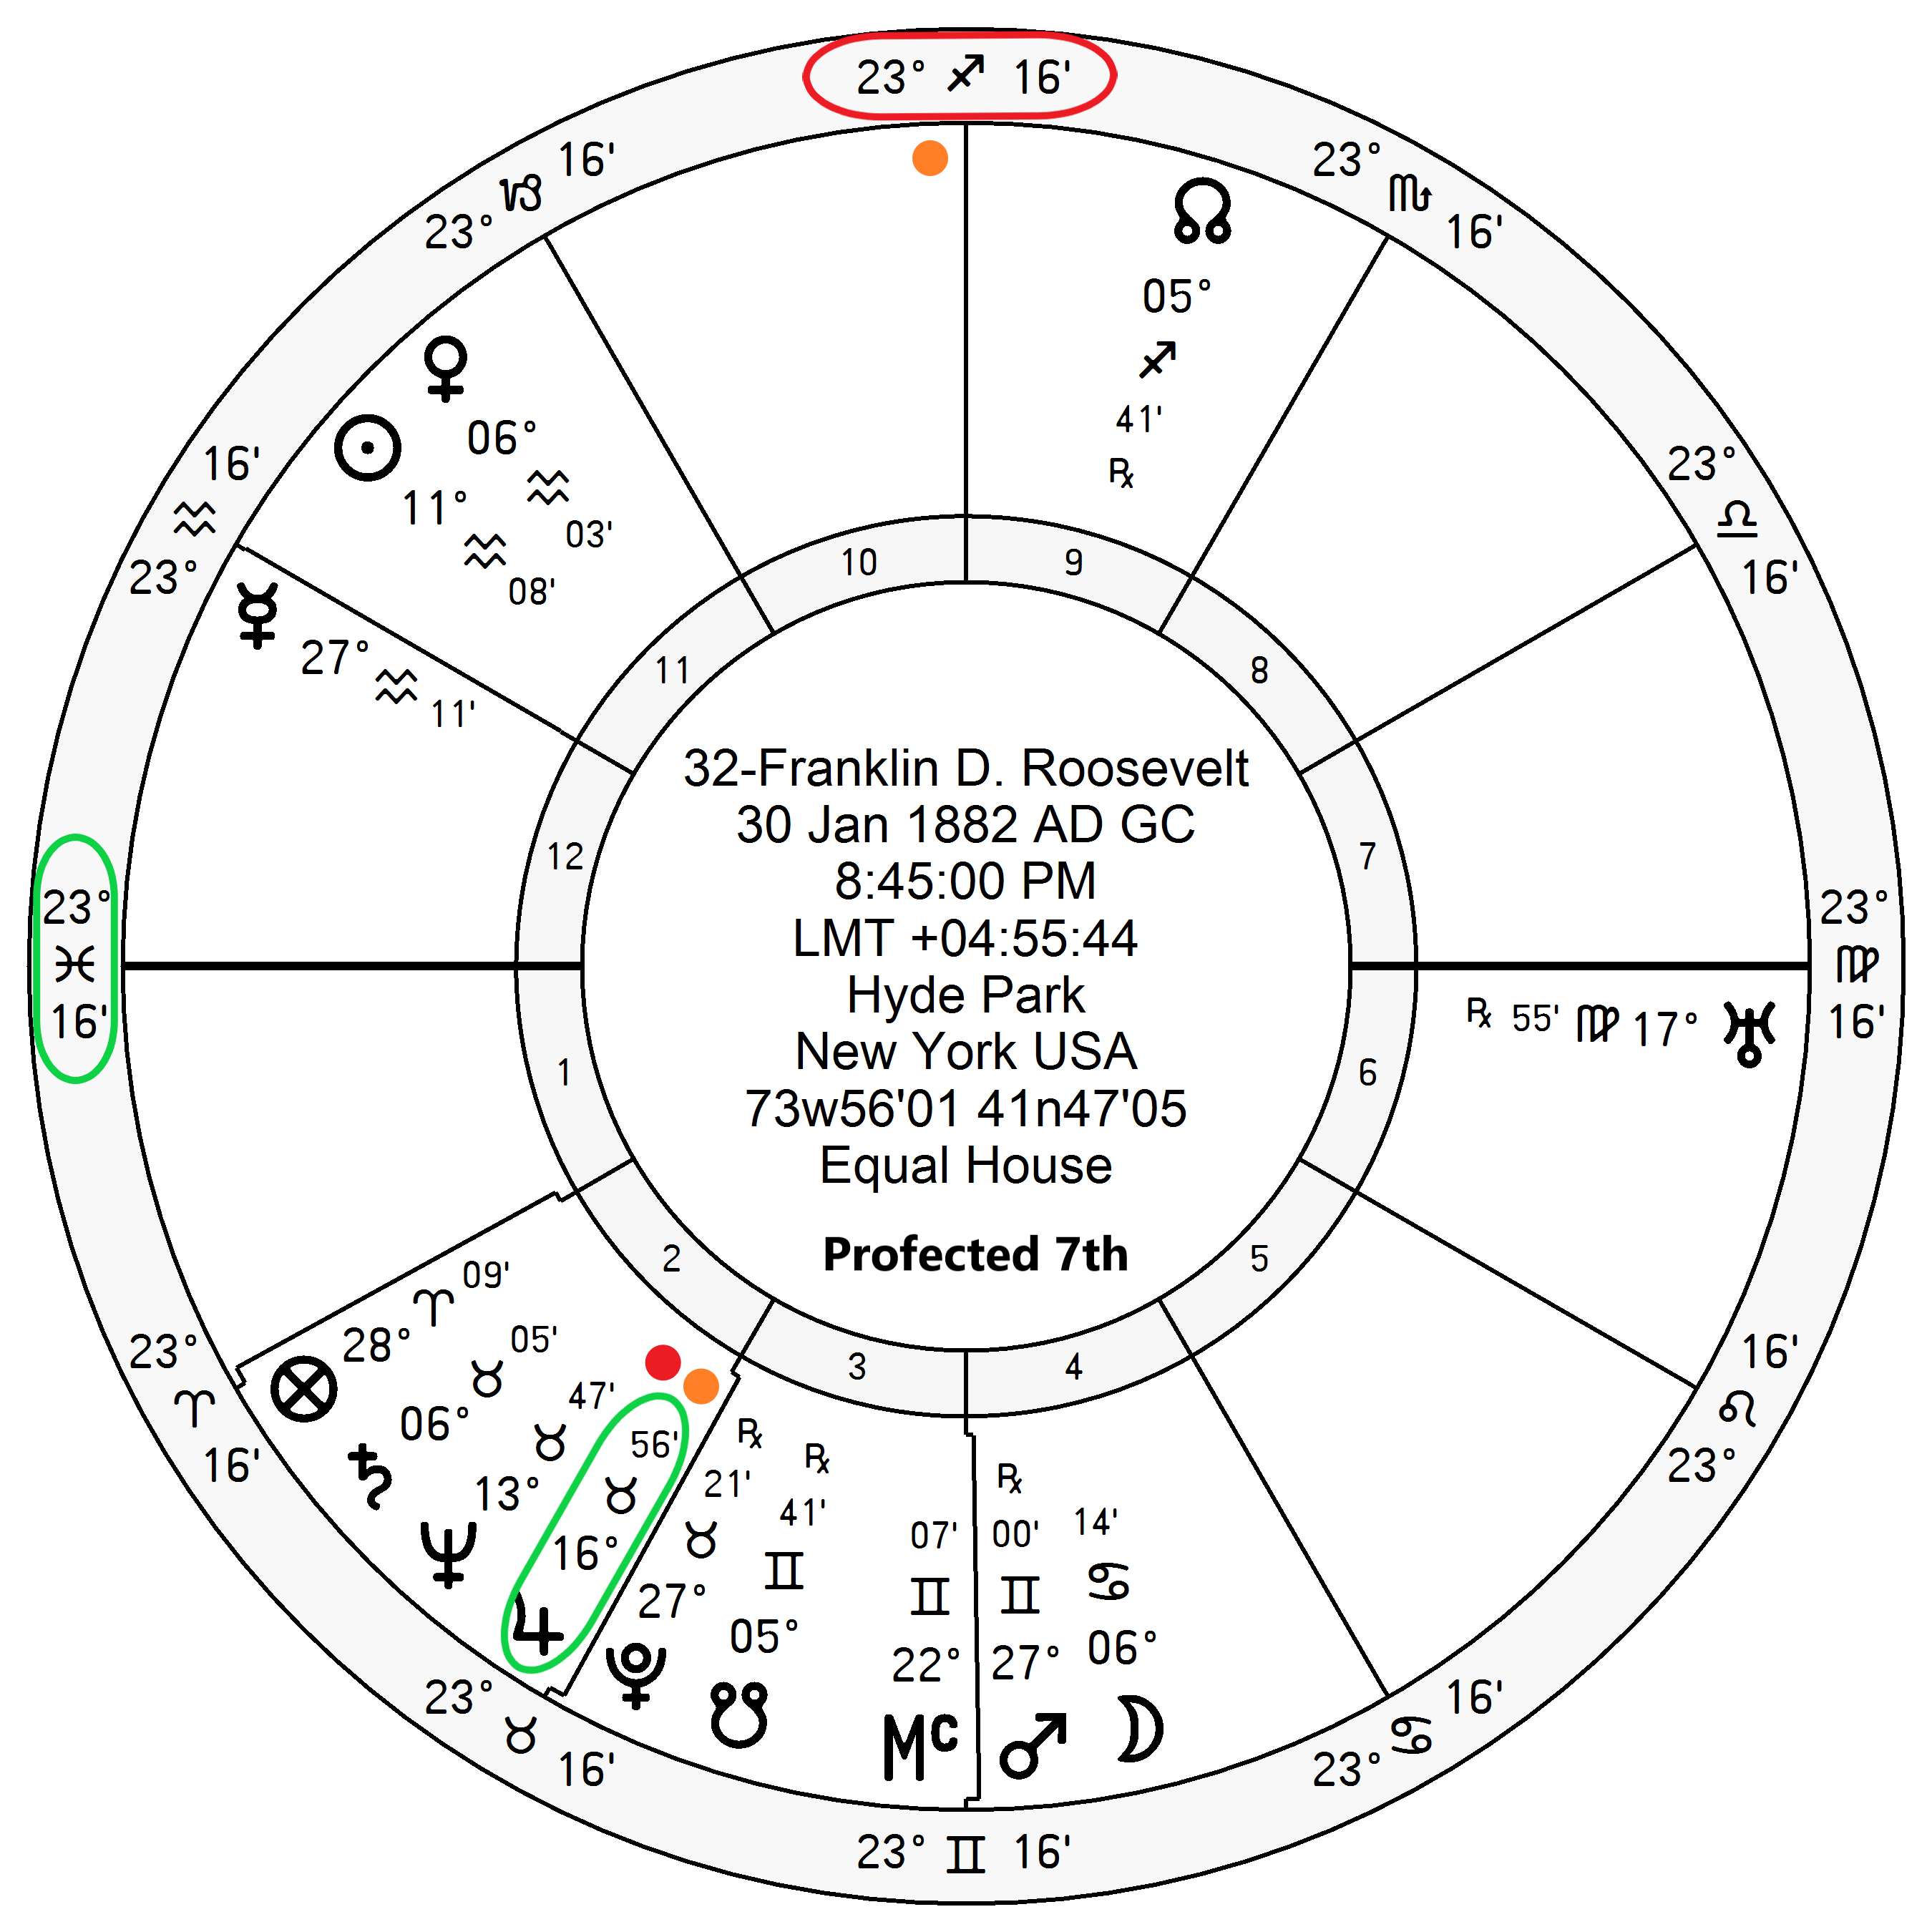
\includegraphics[width=0.9\textwidth]{charts/FDR-Prof-7th.png}}

\textbf{\dgreen P1}=N7
	$\Rightarrow$ \Jupiter\, $\Rightarrow$ \textbf{\dgreen P2/N8} \\
\textbf{\red P10=N4}
	$\Rightarrow$  \Jupiter\, $\Rightarrow$ \textbf{\dgreen P2/N8} \\
PE=\textbf{\red P10/N4}
	$\Rightarrow$  \Jupiter\, $\Rightarrow$   \textbf{\dgreen P2/N8}


\end{columns}
\end{frame}

% candidate
\begin{frame}[t]{Election November 3, 1936: Alf Landon}
\small
\begin{columns}[T, onlytextwidth]
\column{0.48\textwidth}
\vspace{-1em}
{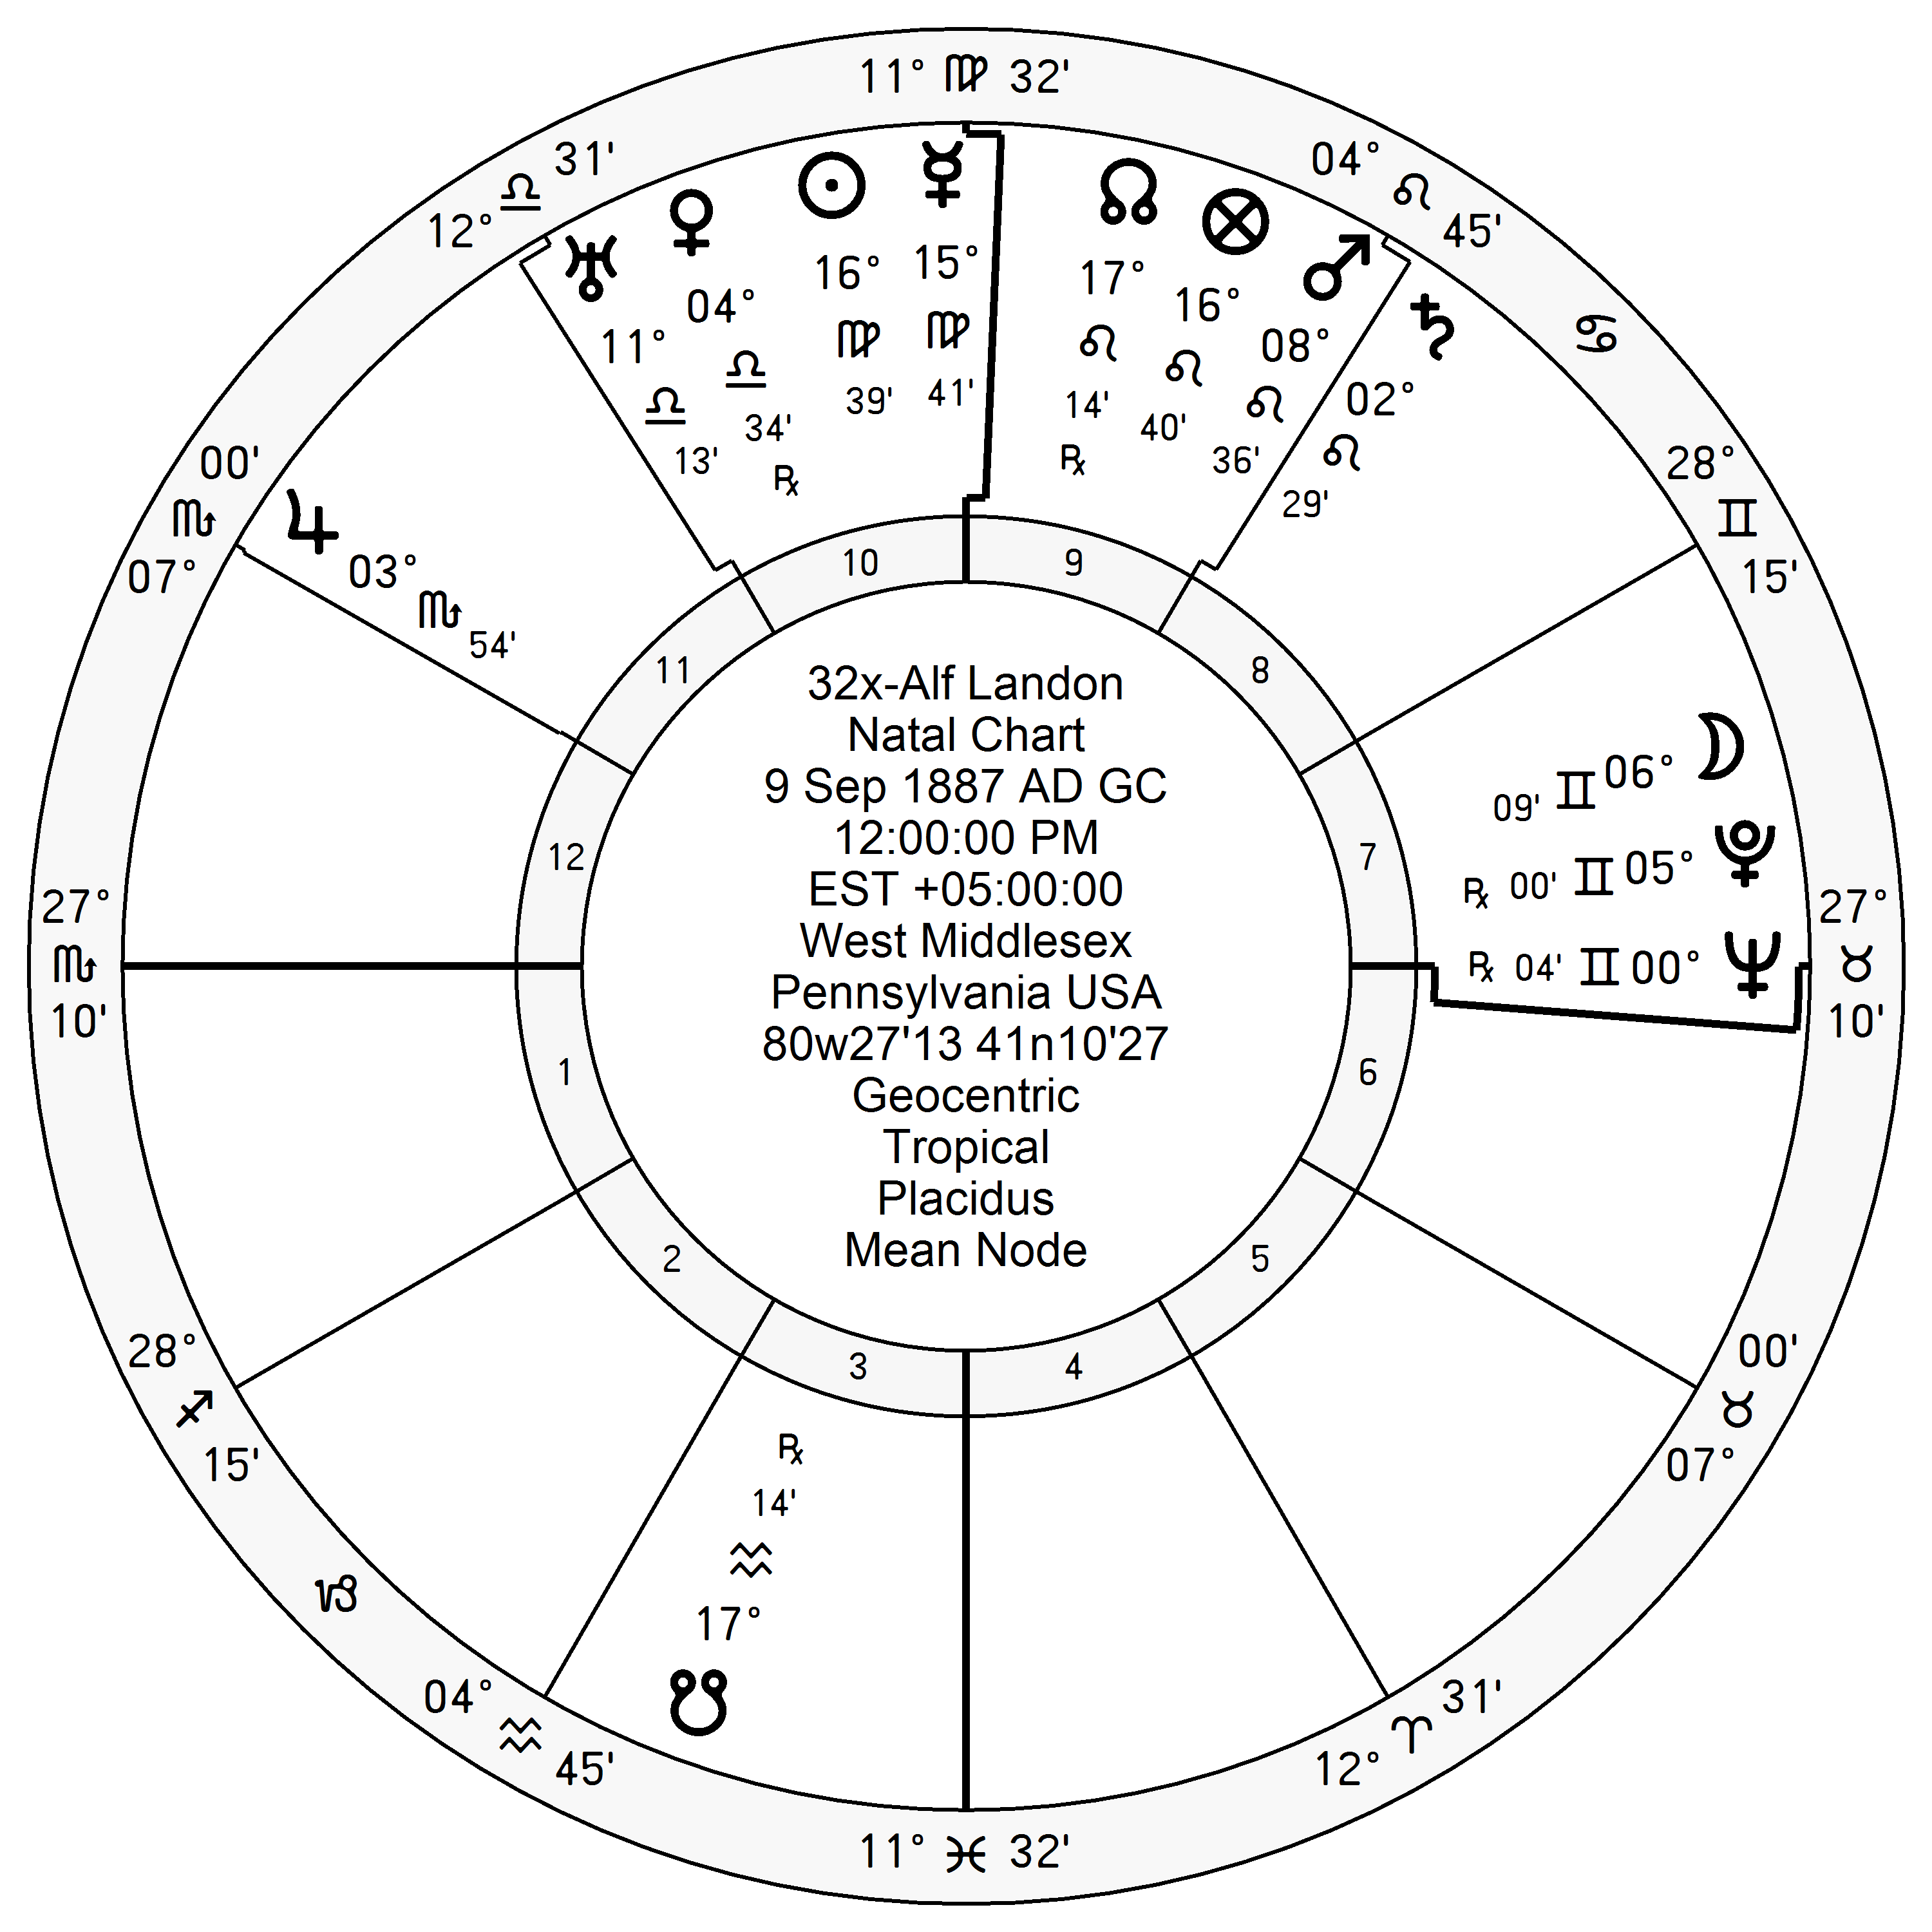
\includegraphics[width=0.9\textwidth]{charts/Landon.png}}
\fontsize{8pt}{9pt}\selectfont

\Jupiter\, \Sextile\, P1 \\
\Mercury\, (burnt) \Trine\, P1 in N10; \Square\, N1 \\
\Saturn\, \Sextile\, P10


\column{0.48\textwidth}
\vspace{-1em}
{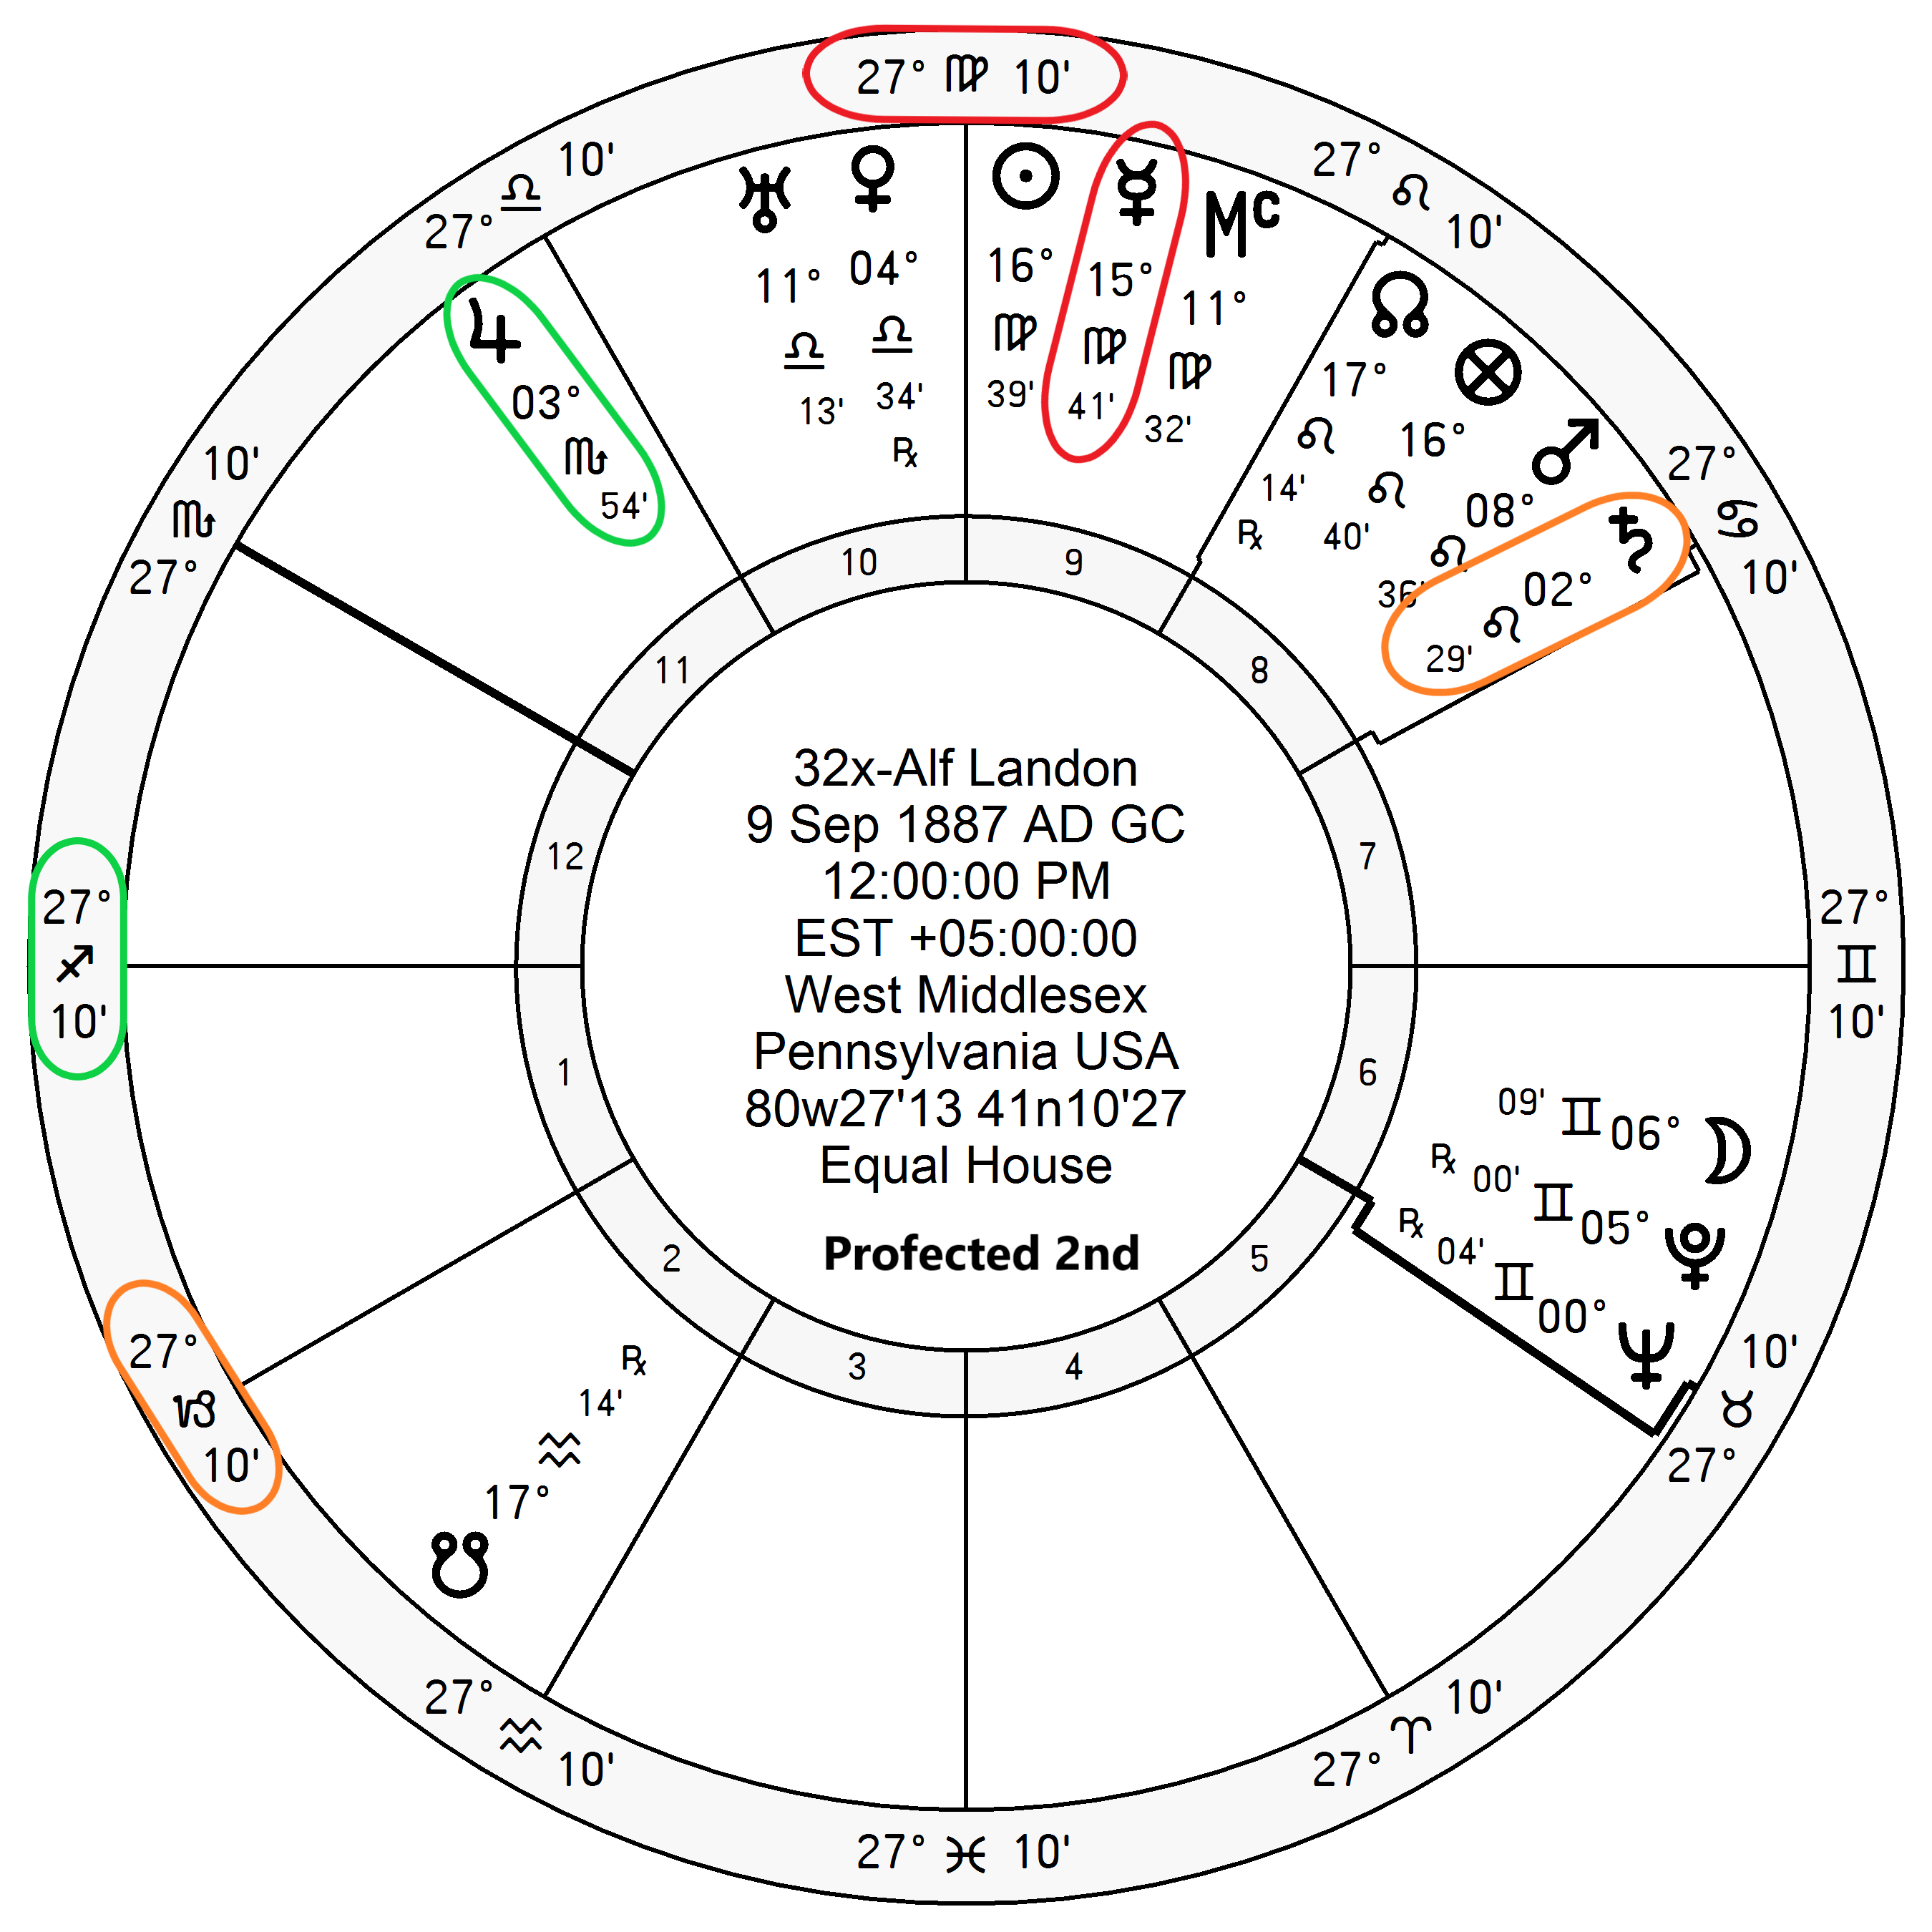
\includegraphics[width=0.9\textwidth]{charts/Landon-Prof-2nd.png}}

\textbf{\dgreen P1=N2} 
	$\Rightarrow$ \Jupiter\, $\Rightarrow$ P11/N11\\
\textbf{\red P10=N10}
	$\Rightarrow$ \Mercury\, (combust) $\Rightarrow$ P9/\textbf{\red N10}\\
PE=P2/\textbf{\dgreen N2}
	$\Rightarrow$ \Saturn\, $\Rightarrow$ P8/N8

\end{columns}
\end{frame}
